\section{Task 2 - Public-Key Authentication in SSH}

\subsection{GNU/Linux}
To generate the ssh-key pair I used the command \verb|ssh-keygen| which generates by default a 2048 bit long rsa key. \\

\begin{figure}
	\centering
	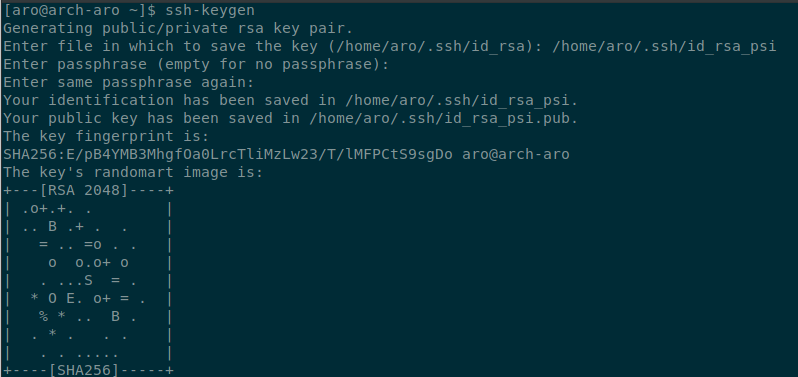
\includegraphics[width=0.8\textwidth]{Assignment0x01/image/ssh-keygen}
	\caption{ssh-keygen} \label{img:key-gen}
\end{figure}

To copy the key on the server \verb|ssh-copy-id user@88.99.184.129| was used. Since I already had a public key for another server and the exercise was to create one, both keys got uploaded to the server as seen in the picture \ref{img:ssh-copy-id}.

\begin{figure}
	\centering
	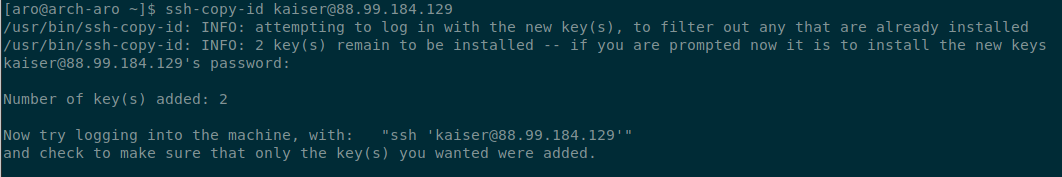
\includegraphics[width=0.8\textwidth]{Assignment0x01/image/ssh-copy-id}
	\caption{save public key on server} \label{img:ssh-copy-id}
\end{figure}

The following log-in worked without the user password for the server. Only the optional password for the private ssh key was required. The keys on the server are stored in \verb|~/.ssh/authorized_keys|. See figure \ref{img:key_server}
\begin{figure}
	\centering
	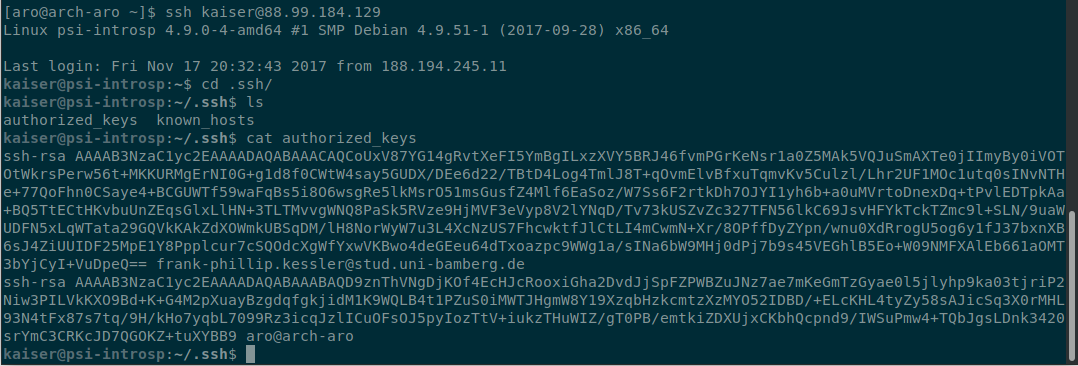
\includegraphics[width=0.8\textwidth]{Assignment0x01/image/ssh_login_key_path}
	\caption{location of keys on server} \label{img:key_server}
\end{figure}

The ssh-keys on your local machine are by default stored in \verb|~/.ssh/id_rsa.pub| for the public part and the private one in \verb|~/.ssh/id_rsa|. (Provided you did create a rsa key) See figure \ref{img:key_local}.

\begin{figure}
	\centering
	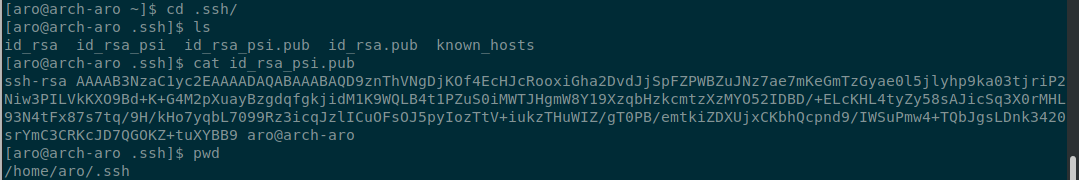
\includegraphics[width=0.8\textwidth]{Assignment0x01/image/ssh_key_local}
	\caption{location of keys on local machine} \label{img:key_local}
\end{figure}

\subsection{Windows}
On a windows machine the same tools from openSSH were not available. That's why the procedure was a little bit different. Here PuTTY was used.

To generate the key the tool \verb|putty-gen| was used.
Then we logged into the server via ssh and created the file \verb|authorized_keys| in \verb|~/.ssh/| and pasted the key into it using nano. Lastly, we checked that only we have write access to the file by \verb|ls -l|

\begin{figure}
	\centering
	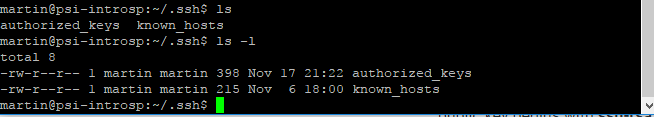
\includegraphics[width=0.8\textwidth]{Assignment0x01/image/jan_2}
	\caption{permission check}
\end{figure}

In figure \ref{img:win_ssh_login} you can see the successful login by using the ssh-key pair.
\begin{figure}
	\centering
	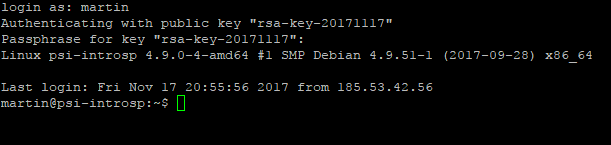
\includegraphics[width=0.8\textwidth]{Assignment0x01/image/jan_3}
	\caption{windows ssh-key login} \label{img:win_ssh_login}
\end{figure}